\chapter{Other methods}

\textbf{hill climbing ok, SA y OpenMP faltan}

Here other possible optimizations are considered that could be used to, in the future, extend the algorithm and perhaps improve its performance and accuracy.

\section{Hill Climbing}

explicar que no es hill climbing exactamente, algo mas simple rollo greedy 
Using the previous optimization we can see a plot of all the possibilities the algorithm considers:

\begin{figure}[!htb]
	\begin{centering}
		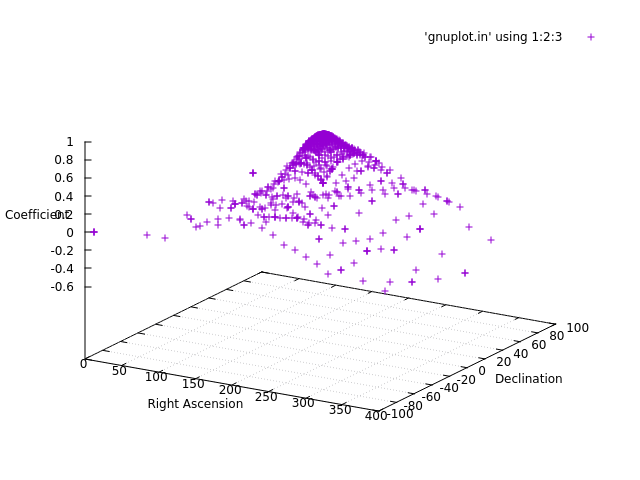
\includegraphics[width=0.5\linewidth]{images/ch6/hillClimbing/resultsAll.png}
		\caption{All visited candidates of the solution space}
		\label{fig:solutionSpace}
	\end{centering}
\end{figure}

As we can see in the previous figure, there appears to be a "hill" (our solution) so an attempt to solve the problem using a \textit{Hill Climbing} approach was also considered.

While not exactly Hill Climbing, a simple greedy algorithm was implemented as a first attempt to test if this method could yield good results:

\begin{minipage}{\linewidth}
	\begin{lstlisting}[language=c, caption=Hill Climbing]
	// Starting position
	sourceInfo current;
	current.ra = 160;
	current.dec = -20;
	int i = 0;
	// Loop with limit or until no progress can't be made
	while (++i < 100) {
		vector<sourceInfo> candidates = getNeighbourList(current);
		sourceInfo newCandidate = getBestCandidate(candidates);
		if (newCandidate < current) {
			break;
		}
		current = newCandidate;
	}
	\end{lstlisting}
\end{minipage}

The following figure shows the results of the execution for two different starting states. For both of them, the algorithm ran until it couldn't progress any further (wasn't interrupted by the iteration limit). The plots contain both the possibilities considered by the decrease range method (in purple, the same plot as \ref{fig:solutionSpace}) and the path taken by the Hill Climbing method (in green).

\begin{figure}[!htb]
	\begin{subfigure}[b]{0.5\textwidth}
		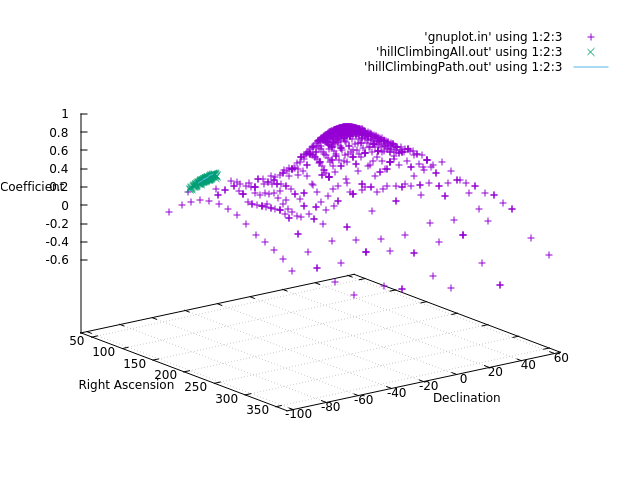
\includegraphics[width=\linewidth]{images/ch6/hillClimbing/resultsPathBad.png}
		\caption{Start: ra=100$^{\circ}$, dec=-60$^{\circ}$}
	\end{subfigure}
	\hfill
	\begin{subfigure}[b]{0.5\textwidth}
		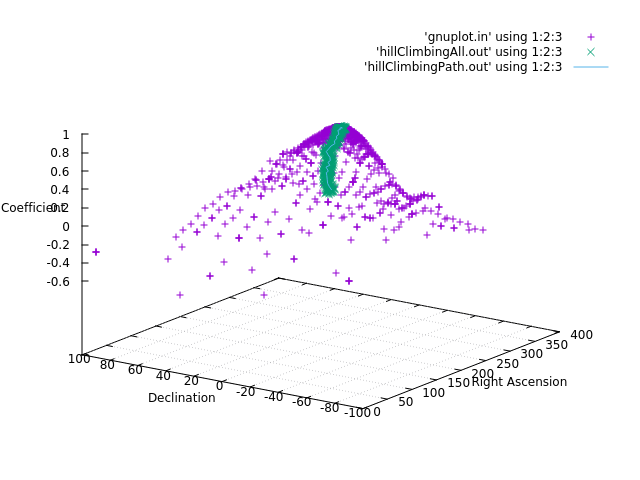
\includegraphics[width=\linewidth]{images/ch6/hillClimbing/resultsPathGood.png}
		\caption{Start: ra=160$^{\circ}$, dec=-20$^{\circ}$}
	\end{subfigure}
	\caption{Paths taken by the Hill Climbing algorithm}
	\label{fig:hillClimbingPaths}
\end{figure}

Visually, we can see that the number of considered possibilities is inferior and the top is reached for case (b), but a problem appears: \textbf{a local maxima}.

If we take a starting right ascension of 160$^{\circ}$ and a declination of -20$^{\circ}$, the algorithm takes a path that gets to the top of our solution, yielding similar results to the previous, decrease range method.

However, with a starting right ascension of 100$^{\circ}$ and a declination of -60$^{\circ}$, the algorithm finds a local maxima on its way and can't progress to the real best solution.

As a result, we can't rely on the Hill Climbing approach for all cases, considering that local maxima may exist for our type of problem. Because of this, another possibility would be to use the Simulated Annealing algorithm so that we can explore other parts of the solution space and find other paths that might lead to our desired solution, instead of only.

\section{Simulated Annealing}

\section{OpenMP}

Explicar OpenMP

\section{Discarding the Sun hemisphere}

So far the algorithm has been studied for the case of the Sun, as it is a source that should be detected more easily than far-away stars. 

The main idea is that the algorithm should detect extraterrestrial EUV sources (if possible) other than the Sun. it follows that it should, before any other computations, discard the Sun hemisphere based on the current Sun location. The greater impact of the Sun's radiation due to its proximity would blind the algorithm from detecting sources that may be having an effect on that hemisphere because of the noise.


explicar como se hace el discard hemisphere

This will be used in the next chapter, in which the presented methods will tested with flares from the Sun and far-away stars.